\documentclass[modern,letterpaper]{aastex61}

% to-do list
% ----------
% - add items here
% style notes
% -----------
% - This file generates by Makefile; don't be typing ``pdflatex'' or some bullshit.
% - Line break between sentences to make the git diffs readable.
% - Use \, as a multiply operator.
% - Reserve () for function arguments; use [] or {} for outer shit.
% - Use \sectionname not Section, \figname not Figure, \documentname not Article or Paper or paper.

% packages
\definecolor{cbblue}{HTML}{3182bd}
\usepackage{microtype}  % ALWAYS!
\usepackage{amsmath,amssymb}
\usepackage{tikz}
\usepackage{aas_macros}
\hypersetup{backref,breaklinks,colorlinks,urlcolor=cbblue,linkcolor=cbblue,citecolor=black}
\graphicspath{{.}{figures/}{../notebooks/plots/}}

% define macros for text
\newcommand{\project}[1]{\textsl{#1}}
\newcommand{\acronym}[1]{{\small{#1}}}
\newcommand{\gaia}{\project{Gaia}}
\newcommand{\rave}{\project{\acronym{RAVE}}}
\newcommand{\apogee}{\project{\acronym{APOGEE}}}
\newcommand{\tmass}{\project{\acronym{2MASS}}}
\newcommand{\documentname}{Article}
\newcommand{\sectionname}{Section}
\newcommand{\figname}{Figure}
\newcommand{\eqname}{Equation}
\newcommand{\dr}{\acronym{DR1}}
\newcommand{\tgas}{\acronym{TGAS}}
\newcommand{\etal}{\textit{et al}.}

\newcommand{\objname}{moving group}
\newcommand{\groupTen}{Group 10}
\newcommand{\groupSixteen}{Group 16}

% define macros for math
\newcommand{\given}{\,|\,}
\newcommand{\normal}{{\mathcal{N}}}
\newcommand{\dd}{\mathrm{d}}
\newcommand{\transp}[1]{{#1}^{\!\mathsf{T}}}
\newcommand{\inv}[1]{{#1}^{-1}}
\newcommand{\bs}[1]{\boldsymbol{#1}}
\newcommand{\vperp}{\bs{v}^\perp}
\newcommand{\propm}{\bs{\mu}}
\newcommand{\mat}[1]{\mathbf{#1}}
\renewcommand{\vec}[1]{\bs{#1}}
\newcommand{\kms}{\ensuremath{\rm km~s^{-1}}}
\newcommand{\msun}{{\rm M}_\odot}
\newcommand{\data}{\mathrm{data}}
\newcommand{\snr}{[S/N]_\varpi}
\newcommand{\eye}{\mathbb{I}}
\newcommand{\absdvtan}{\ensuremath{|\Delta\vec v_\mathrm{t}|}}
\newcommand{\estimates}{\ensuremath{\{\hat{\varpi_i},\hat{\mu_{\alpha,i}},\hat{\mu_{\delta,i}},\hat{v_{r,i}}\}}}

\newcommand{\todo}[1]{{\color{blue}TODO:#1}}

\begin{document}\sloppy\sloppypar\raggedbottom\frenchspacing % trust me

\title{A New? Nearby Young Moving Group -- Latyshev-2 rediscovered?}

\author{Semyeong Oh \etal}

% Affiliations
% \newcommand{\pu}{1}
% \newcommand{\lead}{2}
% \newcommand{\ccpp}{3}
% \newcommand{\mpia}{4}
% \newcommand{\cca}{5}

% \altaffiltext{\pu}{Department of Astrophysical Sciences,
%                    Princeton University, Princeton, NJ 08544, USA}
% \altaffiltext{\lead}{To whom correspondence should be addressed:
%                      \texttt{semyeong@astro.princeton.edu}}
% \altaffiltext{\ccpp}{Center for Cosmology and Particle Physics,
%                      Department of Physics,
%                      New York University, 4 Washington Place,
%                      New York, NY 10003, USA}
% \altaffiltext{\mpia}{Max-Planck-Institut f\"ur Astronomie,
%                      K\"onigstuhl 17, D-69117 Heidelberg, Germany}
% \altaffiltext{\cca}{Center for Computational Astrophysics, 162 5th Ave, New York, NY 10003, USA}


\begin{abstract}
  We characterize two nearby moving groups, \groupTen\ and \groupSixteen,
  using \gaia\ DR 1, data from the literature, and Keck HIRES spectra.
  Notable members include XXX.
  The system is discovered as an aggregate of connected co-moving pairs in our recent study.
  Many of the member stars show signs of youth such as X-ray emission or infrared excess.
  We obtain low resolution spectra of the candidate members selected using proper motions, and
  show that the radial velocities for most of the candidates are indeed consistent
  with sharing the same velocity.
  The proximity of this \objname\  makes it an interesting place to study (special type of stars),
  and look for direct imaging planets.
\end{abstract}

\section{Introduction} % (fold)
\label{sec:introduction}

Stars form in group, and remain coherent in their kinematics for a period of
time that, most importantly, depends on the mass of the initial mass of the
molecular clouds. Thus, looking for comoving groups of stars is an efficient
way to find moving groups of presumably single stellar population.

Simple stellar populations are useful for many things. Based on the assumption
that a group of stars have the same age, many of the stellar parameters can be
more precisely inferred. Particularly, stellar ages, which are important yet
challenging to constrain for a single star, can be pinned down to
\todo{$approx 10$\%} precision.

Young, hot stars are primary targets for discovering planets and brown dwarfs
with direct imaging.

Here, we report extended analysis and spectroscopic characterization of two
nearby moving groups.

\subsection{Previous identifications}
\label{subsec:history}

Moving group identifications are often scattered throughout the literature.
From a (non-exhaustive) bibliography review of all \tgas\ sources associated
with \groupTen\ and \groupSixteen\ using Simbad database, we note previous
identifications of these groups in the literature.

Some A-type stars that were selected in \citet{2017AJ....153..257O} as potential
members of \groupTen, 84 Uma, 81 Uma, XXX, were previously suggested by
Latyshev77




% section introduction (end)

\section{Observation}
\label{sec:observation}

\subsection{Target Selection}
\label{sub:target_selection}

We re-examined the network of co-moving pairs studied in \citealt{2017AJ....153..257O} by
lowering the threshold of the marginalized likelihood ratios to be more inclusive.
For $\ln{\mathcal{L}_1}/{\mathcal{L}_2}>2$, we find that this group,
identified as group id 10 in \citealt{2017AJ....153..257O}, is extended to 45 potential members.

table for targets and observation

\section{Searching lower main sequence in GPS1}
\label{sec:searching_lower_main_sequence_in_gps1}

% \begin{figure}[htpb]
%   \centering
%   \includegraphics[width=0.8\linewidth]{g0_pm.pdf}
%   \caption{
%     Group 0 (the Pleiades; black circles) stars in proper-motion space. The
%     stars are well-separated from the distribution of the background stars
%     within the same patch of the sky. The Blue box indicates the proper motion
%     cuts applied to select stars from GPS1 catalog.
%   }
%   \label{fig:g0_pm}
% \end{figure}

% \begin{figure}[htpb]
%   \centering
%   \includegraphics[width=0.95\linewidth]{g0_gps1.pdf}
%   \caption{
%     Potential members of the Pleiades selected from GPS1. These are 2095 stars
%     that are within 15 degrees from the center (median RA, Dec) and have proper
%     motions within the cuts indicated in Figure 1 . The line in each panel is
%     the isochrone from MIST model. In the top left panel, the purple shade for
%     the (pre-)main sequence shows the span from using the minimum and the
%     maximum parallax values. In order to shift the model magnitudes to observed
%     magnitudes, a point-estimate distance of 1/(median parallax) is used.
%   }
%   \label{fig:g0_gps1}
% \end{figure}

We first find the lower main-sequence stars of the Pleiades (Group 0) using the
GPS1 data. The Pleiades is chosen as it is clearly very separated in
proper-motion space alone (Figure 1). We apply a simple cut in proper motions
to be within the minimum and maximum values of the TGAS-selected Group 0
members (indicated with a blue box in Figure 1, and query 15 degrees around the
center (median RA, Dec) of the group. There are 2095 stars satisfying the cuts
in the GPS1 catalog. Figure 2 shows their distribution in color-magnitude
diagrams using Gaia, 2MASS, and PanSTARRS photometry with MIST (\citealt{2016ApJ...823..102C}).

We first find the lower main-sequence stars of the Pleiades (Group 0) using the
GPS1 data. The Pleiades is chosen as it is clearly very separated in
proper-motion space alone (Figure~\ref{fig:g0_pm}). We apply a simple cut in
proper motions to be within the minimum and maximum values of the TGAS-selected
Group 0 members (indicated with a blue box in Figure~\ref{fig:g0_pm}, and query 15
degrees around the center (median RA, Dec) of the group. There are 2095 stars
satisfying the cuts in the GPS1 catalog. Figure~\ref{fig:gps_gps1} shows their
distribution in color-magnitude diagrams using Gaia, 2MASS, and PanSTARRS
photometry with the MIST isochrone of solar metallicity and 8.5~Myrs. Although
there is clearly contamination from background stars with this simple cuts, the
expected over-density in the low main-sequence is well recovered (and possibly
a few suspect WDs on the cooling sequence!).

However, there is a noticeable disagreement between the MIST isochrone and the
data in the red colors in that the model isochrone predict bluer colors than
observed. This is a known problem due to incomplete spectral library for
generating stellar spectral energy distributions from physical parameters
(Choi+2016).


We searched the Simbad (\citealt{2000A&AS..143....9W}) database for existing
radial velocity measurements of the candidate members


\section{Discussion}
\label{sec:discussion}

% \begin{deluxetable}{cccccccc}
\tablecaption{Candidate members of the new moving group}
\tablehead{\colhead{Id} & \colhead{RA} & \colhead{Dec} & \colhead{$d$} & \colhead{$\mu_\alpha^*$} & \colhead{$\mu_\delta$} & \colhead{$G$} & \colhead{$G-J$}\\ \colhead{ } & \colhead{$\mathrm{{}^{\circ}}$} & \colhead{$\mathrm{{}^{\circ}}$} & \colhead{$\mathrm{pc}$} & \colhead{$\mathrm{mas\,yr^{-1}}$} & \colhead{$\mathrm{mas\,yr^{-1}}$} & \colhead{$\mathrm{mag}$} & \colhead{$\mathrm{mag}$}}
\startdata
TYC 4164-274-1 & 204.86346 & 61.06173 & 102 & -18.34204 & -4.19466 & 11.72 & 1.54 \\
TYC 3471-333-1 & 210.58975 & 52.41774 & 94 & -12.38721 & -5.52270 & 10.15 & 1.12 \\
TYC 3480-1209-1 & 223.27004 & 51.26115 & 103 & -14.19318 & -0.68498 & 9.77 & 0.97 \\
HIP 69650 & 213.82070 & 52.53591 & 96 & -17.60329 & -3.47382 & 6.57 & 0.21 \\
TYC 3489-1148-1 & 234.45997 & 51.53768 & 105 & -11.96797 & -0.04552 & 10.79 & 1.24 \\
TYC 3470-485-1 & 206.31849 & 52.24726 & 101 & -14.23060 & -1.42733 & 10.36 & 1.33 \\
TYC 3851-336-1 & 205.40212 & 53.33751 & 100 & -18.00650 & -3.34968 & 9.54 & 0.96 \\
TYC 3868-177-1 & 230.81618 & 54.84823 & 112 & -13.79247 & -1.23381 & 10.89 & 1.28 \\
TYC 3867-127-1 & 225.82014 & 59.01152 & 102 & -12.24411 & -4.24575 & 9.24 & 0.84 \\
HIP 72389 & 222.01173 & 56.15920 & 98 & -15.86543 & -1.52228 & 9.75 & 1.15 \\
TYC 3851-369-1 & 205.78236 & 54.02590 & 96 & -19.00362 & -2.86724 & 9.49 & 0.96 \\
TYC 3490-1083-1 & 237.50530 & 45.92063 & 106 & -2.20292 & -7.24028 & 10.77 & 1.17 \\
HIP 73730 & 226.07328 & 59.53505 & 112 & -13.66060 & -0.16444 & 7.38 & 0.31 \\
TYC 3471-233-1 & 211.95507 & 51.95266 & 100 & -16.80352 & -4.58756 & 11.01 & 1.34 \\
TYC 3486-1405-1 & 234.13473 & 48.27970 & 104 & -7.18765 & -2.91899 & 11.13 & 1.30 \\
TYC 3860-1483-1 & 219.85980 & 54.77406 & 91 & -17.56146 & -2.79769 & 9.62 & 1.00 \\
TYC 3877-725-1 & 240.27846 & 53.41640 & 116 & -9.55302 & 0.50717 & 10.15 & 0.98 \\
HIP 71911 & 220.63149 & 60.23096 & 106 & -16.23543 & -3.84032 & 8.02 & 0.60 \\
TYC 4174-1117-1 & 209.67123 & 63.68877 & 94 & -18.90730 & -4.20806 & 10.96 & 1.60 \\
TYC 4173-609-1 & 219.82002 & 61.93126 & 101 & -17.03522 & -3.99511 & 10.20 & 1.04 \\
HIP 74458 & 228.24118 & 56.04643 & 116 & -13.15720 & -1.18896 & 7.50 & 0.40 \\
TYC 3867-1373-1 & 222.87595 & 59.53208 & 104 & -15.36222 & -1.74196 & 11.41 & 1.41 \\
TYC 3867-281-1 & 226.10718 & 59.88078 & 107 & -13.39936 & -0.06820 & 9.46 & 1.01 \\
HIP 68637 & 210.74889 & 50.97178 & 101 & -16.44373 & -6.20977 & 6.18 & 0.11 \\
TYC 3875-762-1 & 231.92341 & 59.98704 & 112 & -13.29654 & 0.09361 & 10.79 & 1.31 \\
TYC 3850-257-1 & 201.21590 & 54.89743 & 90 & -19.01098 & -6.27073 & 7.51 & 0.51 \\
HIP 63702 & 195.81947 & 57.31521 & 98 & -17.10263 & -8.19643 & 8.94 & 0.91 \\
TYC 4180-573-1 & 226.31493 & 60.70688 & 107 & -14.94724 & 3.30343 & 11.41 & 1.73 \\
HIP 66198 & 203.53030 & 55.34841 & 95 & -19.07864 & -6.07010 & 5.65 & 0.05 \\
HIP 69275 & 212.72088 & 62.52220 & 104 & -17.16634 & -3.03405 & 8.18 & 0.70 \\
HIP 75449 & 231.20862 & 51.21025 & 104 & -9.45363 & 1.95656 & 8.71 & 0.86 \\
TYC 3851-600-1 & 207.11420 & 54.04270 & 94 & -18.28773 & -3.93385 & 10.72 & 1.29 \\
TYC 3861-1374-1 & 222.52355 & 53.63483 & 104 & -14.56375 & -1.91517 & 10.04 & 1.10 \\
TYC 3865-934-1 & 216.29630 & 57.63321 & 105 & -15.38139 & -2.48544 & 9.49 & 0.86 \\
HIP 67231 & 206.64844 & 54.43266 & 98 & -18.53300 & -4.75037 & 5.72 & 0.02 \\
HIP 69917 & 214.62966 & 52.03331 & 100 & -17.19397 & -3.12164 & 6.91 & 0.32 \\
HIP 78958 & 241.78394 & 49.08308 & 114 & -13.79672 & -2.60256 & 7.57 & 0.41 \\
TYC 3869-656-1 & 232.80915 & 53.46013 & 108 & -12.59986 & -0.73862 & 11.25 & 1.33 \\
HIP 69958 & 214.73284 & 54.86376 & 104 & -16.56509 & -2.06314 & 6.45 & 0.35 \\
HIP 77903 & 238.64981 & 49.39545 & 112 & -11.66980 & -1.48668 & 9.73 & 0.90 \\
TYC 3496-1082-1 & 237.92411 & 52.30631 & 118 & -10.69995 & -1.47975 & 11.23 & 1.33 \\
TYC 3497-1053-1 & 240.51009 & 51.33533 & 120 & -10.45759 & 0.90600 & 11.08 & 1.24 \\
TYC 3867-2-1 & 226.27980 & 57.51270 & 120 & -13.18434 & -1.65660 & 11.05 & 1.57 \\
HIP 67005 & 205.97812 & 52.06439 & 93 & -18.27010 & -5.60471 & 6.05 & 0.10 \\
HIP 69721 & 214.07256 & 58.38940 & 107 & -16.25440 & -2.90256 & 8.40 & 0.70
\enddata

\tablecomments{some shit}

\end{deluxetable}



% \begin{figure}[htpb]
%   \centering
%   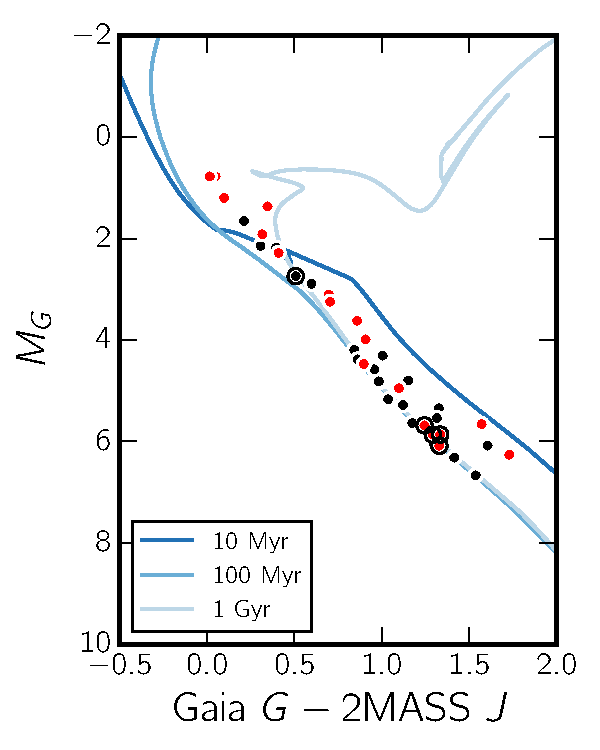
\includegraphics[width=0.7\linewidth]{cmd_gjg.pdf}
%   \caption{Color-magnitude diagram of member stars.
%     For comparison, we show the MIST isochrones of a solar metallicity population \todo{cite mist}.
%     Red markers indicate infrared excess,
%     and markers wrapped in black circles indicate X-ray source (Table~\todo{tablenum}).
%   }
%   \label{fig:cmd_gjg}
% \end{figure}

\acknowledgements
% simbad
This research has made use of the SIMBAD database,
operated at CDS, Strasbourg, France.
% ads
This research has made use of NASA's Astrophysics Data System.


\bibliography{refs}

\end{document}
